\section{Results} \label{Results}

\subsection{Main Results}

Figure \ref{ResultsPlot} shows estimated dynamic treatment effects and 95\% confidence intervals for all students and the four subgroups of interest. Note that the precision of the estimates tends to decrease with the distance in time from treatment. Recall that the number of observed units decreases with the distance in time from treatment (see Table \ref{tab:BinSizes}). The reason for this is that in order to experience eight treated years, the county has to experience its first disaster very early. Similarly, it has to receive treatment very late to experience more than five years before treatment. As a result, the uncertainty increases with the distance in time from treatment.

\begin{figure}[!h]
	\centering
	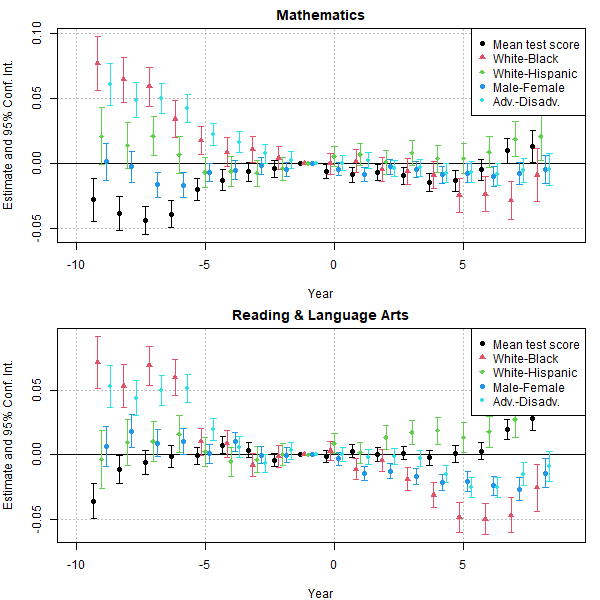
\includegraphics[scale=1]{"../Code & Data/ResultsPlot.pdf"}
	\caption{Dynamic Treatment effects in relative time: FEMA disaster data}
	\label{ResultsPlot}
\end{figure}

For the period of treatment there is a significant\footnote{Significant is used here in the sense that a confidence interval with nominal coverage of 95\% does not include zero, that is a corresponding t-test would reject the null hypothesis of a zero effect at the 5\% level.} effect of natural disasters on the performance in mathematics. Also, one year after the disaster there is an even larger significant decrease in test scores. For all subsequent periods the effect on mathematics scores is not significant. For RLA scores, on the other hand, we see significantly positive effects after three years. In other words, RLA test scores actually tend to improve three to five years after a natural disaster.

The estimated effects among the subgroups are relatively similar: Negative effects on mathematics test scores in the short term, but positive long-term effects in RLA. For black and hispanic students, however, we do not even find the negative effects on mathematics, but among black students there is a significant decrease in mathematics scores after five years.

The effect sizes for the short-term effect range from barely above zero to about -0.02 standard deviations of the national reference cohort. The positive long term effects go up to 0.05 standard deviations of the national reference cohort. Here, the effect on black and hispanic students seems to be larger than on white students. Also, female students seem to be more positively affected. Their test scores improve by between 0.02 and 0.04 standard deviations of the national reference cohort four or five years after the disaster.

The positive medium- and long-term effects may be surprising, but positive effects of disasters on performance are not unheard of in the literature. In fact, this is somewhat consistent with the findings by \cite{Sacerdote_2012}, who attributes them to student mobility after the disaster. Due to destroyed infrastructure, many students have to switch schools and some may even benefit from attending a higher quality school after the disaster. Thus, if a disaster leads to students switching from lower quality to higher quality schools, positive effects are very plausible.

Figures \ref{ResultsPlotStorm} shows the same graphs based on the storm treatment. Overall, we also find a significantly negative effect on mathematics test scores in the same year.

\begin{figure}[!h]
	\centering
	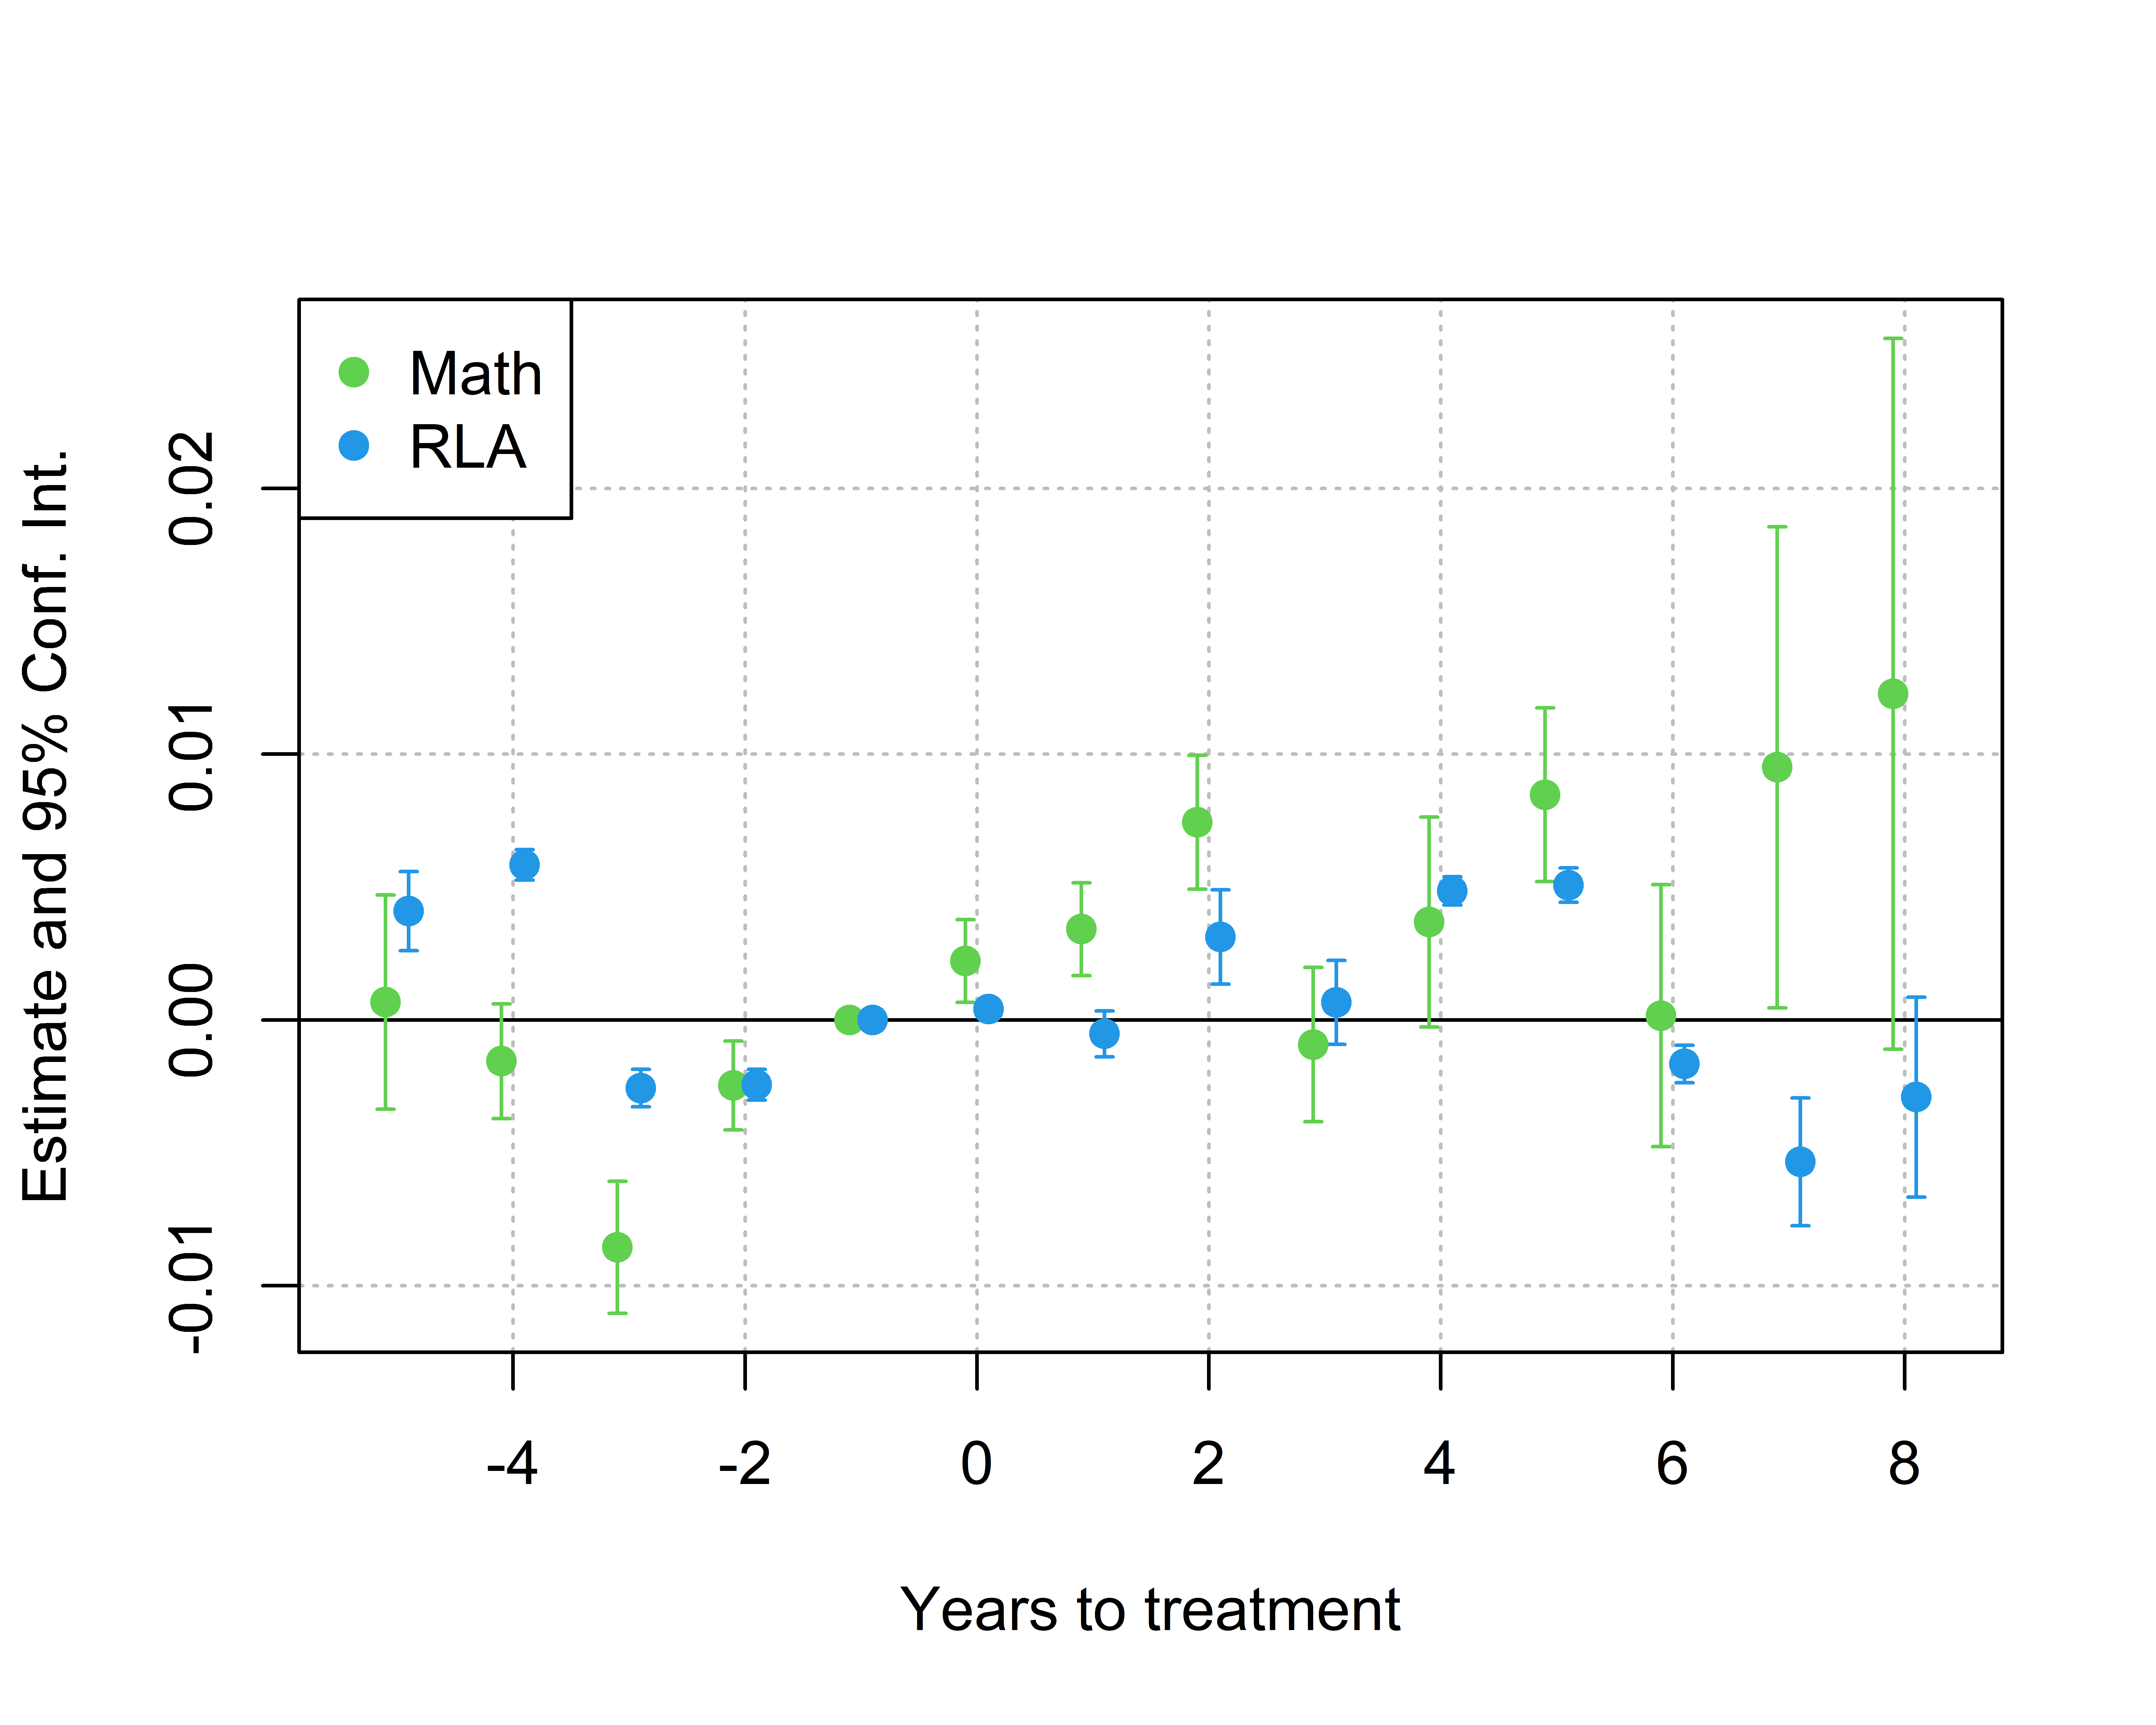
\includegraphics[scale=1]{"../Code & Data/ResultsPlotStorm.pdf"}
	\caption{Dynamic Treatment effects in relative time: NWS storm data}
	\label{ResultsPlotStorm}
\end{figure}

Similarly, white students experience a significant decline in mathematics scores in the same year, but they see an improvement in RLA scores three to five years after the disaster. For other subgroups, however, we do not find this effect in the storm data. For black and hispanic students, we find no significant effects, while for female and disadvantaged students we find a significant decrease in both mathematics and RLA.

\subsection{Heat Results}

Table \ref{tab:HeatResults} provides the estimation results for the heat models. Rows 1 and 2 show the estimated coefficients and standard errors for the maximum temperature variable for mathematics and RLA respectively. We find a significant effect of daily maximum temperature on mathematics scores. This is also significant and more pronounced among hispanic, female and, economically disadvantaged students. The effect on RLA is only significant among black students. Based on these point estimates, a year that is 5-10°C hotter has a similar effect as a natural disaster.


\begin{tabular}{lllllll}
\toprule
  & Overall & White & Black & Hispanic & Female & Econ. Disadv.\\
\midrule
Max. Temp. (Math) & $-0.0007$ & $-0.0002$ & $-0.0006$ & $-0.0021^{***}$ & $-0.001^{***}$ & $-0.0011^{***}$\\
 & $(0.0003)$ & $(0.0004)$ & $(0.0008)$ & $(0.0006)$ & $(0.0004)$ & $(0.0004)$\\
\addlinespace
Max. Temp. (RLA) & $-0.0001$ & $0.0005$ & $-0.0015^{***}$ & $-0.0011^{***}$ & $-0.0002$ & $-0.0004$\\
 & $(0.0003)$ & $(0.0003)$ & $(0.0007)$ & $(0.0006)$ & $(0.0003)$ & $(0.0003)$\\
\addlinespace
Days ab. 30 (Math) & $-0.000169$ & $-0.000111$ & $0.000033$ & $-0.000196$ & $0.000003$ & $0.000003$\\
 & $(0.000089)$ & $(0.000096)$ & $(0.000143)$ & $(0.000136)$ & $(0.000095)$ & $(0.000096)$\\
\addlinespace
Days ab. 30 (RLA) & $-0.000095$ & $-0.000178^{***}$ & $-0.00014$ & $-0.000483^{***}$ & $-0.000202^{***}$ & $-0.000027$\\
 & $(0.000071)$ & $(0.000079)$ & $(0.000122)$ & $(0.000117)$ & $(0.000079)$ & $(0.000079)$\\
\addlinespace
\midrule
Mean & -0.042 & 0.107 & -0.483 & -0.281 & 0.025 & -0.284\\
\bottomrule
\end{tabular}


Rows 3 and 4 of Table \ref{tab:HeatResults} show the same results for the number of days above 30°C. Here, we only find a significant effect on RLA among white, hispanic and female students in RLA. For hispanic students the point estimate is $-0.0004$, meaning about 25 additional days above 30°C would be somewhat comparable to the average effect of a natural disaster in the same year, a rather small effect. For white and femal students, the effect size is even smaller.

In total, we find only limited evidence for a negative effect of heat on the achievement in standardized tests. However, it seems to be more pronounced among some subgroups. For hispanic students the point estimates are substantially larger when significant. This is somewhat consistent with other authors' findings \citep[for example][]{Goodman_2020}

One explaining factor could be the presence of air-conditioning. The results in \cite{Goodman_2020} suggest that air conditioning offsets about three quarters of the negative effect of heat exposure. Possibly, counties with higher shares of minority students tend to have a lower presence of air-conditioning in schools. Also, black and hispanic households tend to be poorer on average and may therefore be less likely to have air-conditioning at home. This could explain some of the heterogeneity in the effect of heat.

\subsection{Discussion}

Based on the FEMA data, there are negative short-term effects but positive long-term effects of disasters on academic achievement. The NWS storm data, on the other hand, does not support this. Here, we only find positive effects among white students in RLA. However, this does not seem to be driven by heterogenity of disaster types. Repeating the same analysis using only the storms in the FEMA dataset (see Appendix \ref{AppendixA}) does not lead to the same conclusion. In fact, those results are more similar to the original FEMA results. This is rather unexpected. It turns out the overlap between the storms in the FEMA and the NWS dataset is pretty small: Only 192 of about 5000 storms could be unambigously matched by county and date. This suggests that there may be some severe inconsistencies in either the FEMA or the NWS data on storms.

Our effect sizes for the short-term effects are consistently around -0.01 or -0.02. Recall that these values are measured on the cohort standardized scale, that is they measure the distance from a national reference cohort in standard deviations of that national reference cohort. To compare the effect size to that of other studies it makes sense to standardize it differently. By dividing through the sample standard deviation we can standardize the results with respect to the other students in the sample. This results in a (roughly) 3-4 fold increase of the effect sizes (see Table \ref{tab:SumStats}). Even after this 3-4 fold increase, our effect sizes seem to be rather small. For example, \cite{Sacerdote_2012} finds decreases of 0.17 standard deviations in math scores. On the other hand, \cite{Sacerdote_2012}, as well as most of the previous studies, focuses on two very extreme events, namely hurricanes Katrina and Rita, while we use a very comprehensive sample of many disasters. Naturally, the expected effect size should be smaller for the latter.

We speculate that some of our results are largely driven by migration responses to disasters. This is a prominent theme in previous studies on disasters and learning \citep{Pane_2008, Sacerdote_2012}. That's why it may be interesting to have a look at the ethnic composition of the counties relative to initial treatment. Figure \ref{EthnicComposition} shows ethnic shares of enrolled students for the treated counties in relative time.

\begin{figure}[!h]
	\centering
	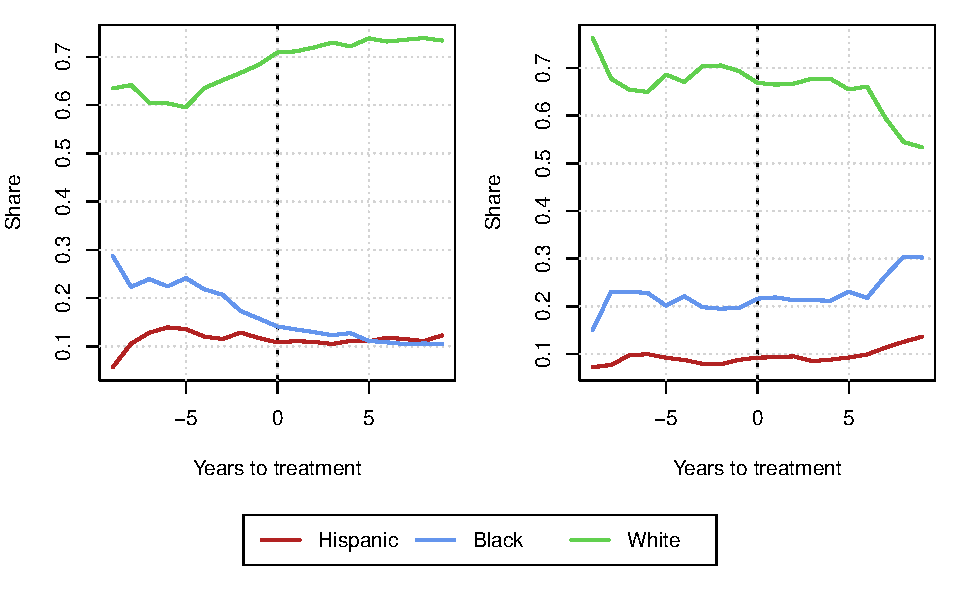
\includegraphics[scale=1]{"../Code & Data/EthnicComposition.pdf"}
	\caption{Aggregated ethnic shares of enrolled students by treatment timing based on FEMA disasters (left) and on NWS storms (right)}
	\label{EthnicComposition}
\end{figure}

In the left panel we see that the share of black students decreases in counties that experienced a disaster around the time of the disaster. This supports the hypothesis that black students disproportionately switch schools after disasters and may explain the positive long term effect as described above. However, the share of black students already decreases before treatment, so this may not be a causal effect of the disaster, but a general demographic trend. This fact could also explain why we do not observe any negative short-term effects among black and hispanic students.

The same plot based on the NWS storm data shows a different picture. Here, all three shares remain somewhat constant until five years after treatment. Then the share of black students increases, while the share of white students decreases. This suggests that the migration response to storms may be qualitatively different than the response to other forms of disasters. At least for the storms data this does not seem to be a major driver of the results.

A more in-depth analysis of migration responses to natural disasters and their role in academic achievement is unfortunately not possible with this data. There is some prior research based on individual level data indicating that it does play an important role \citep[for example][]{Sacerdote_2012}. Analyzing migration responses and their link to academic achievement for different types of natural disasters may be a promising area for future research.

For the heat results, we find some negative effects and substantial heterogeneity: Minorities, especially hispanic students, and disadvantaged students seem to be more prone to adverse effects of heat exposure. Again, we want to compare the effect sizes to other authors. \cite{Park_2020} find overall reductions in test scores of 0.0004 standard deviations and 0.0010–0.0012 standard deviations of an additional hot day. Adjusting our coefficients as above to be in terms of sample standard deviations, we find a slightly higher effect on RLA scores among hispanic students (roughly 0.0012-0.0017 standard deviations). Our overall effect is not significant, but our effect on white students is very close in size to their overall effect. However, their threshold of what classifies as a hot day is slightly lower (26.7°C), so this may drive the differences.

The results in \cite{Goodman_2020} indicate that air-conditioning mitigates a large part of the negative effect. Based on that, we speculate that inequality in air-conditioning is the main driver of said heterogeneity, since minority students tend to have less access to air-conditioning. Improving the air-conditioning coverage in more affected schools could be an easy way for policymakers to adress the adverse effects of heat on academic achievement. However, to the best of our knowledge \cite{Goodman_2020} is the only paper to study this relationship. More research on the interconnection between heat, learning, and air-conditioning may be useful to make policy decisions.

Obviously, our results come with limitations. First, we find significant pre-treatment effects in the FEMA treatment. Therefore, the treatment led to a significant difference in average test scores between treatment and control group before the treatment even began. This is likely caused by a violation of one of the two identifiying assumptions: Either the trends in outcomes of treatment and control group are not parallel or treated units anticipated treatment and therefore already saw an effect earlier. Since the latter is rather implausible, we conclude that there might be a violation of the parallel trends assumption. This is in line with the pre-treatment trends in Appendix \ref{PreTrends} that look better for the NWS data. Thus, the FEMA results should be interpreted with more caution.

Based on the results from Section \ref{Data}, in particular Figure \ref{AssistCovBoxplot}, it seems that there are significant differences between counties that apply for (and receive) federal assistance after a disaster and those that do not. If such federal assistance offsets the negative effect on the education system, our estimates could be biased. However, this would suggest that the effects could be even larger in the absence of federal aid. Therefore, our estimates may only provide a lower bound on the true effect, which could be much larger.

For the heat results, the measures of heat exposure used are based on daily maximum temperature only. However, this likely does not fully capture the physiological impact of heat. Other variables, like humidity or minimum temperatures overnight, can also contribute to the negative effect of heat on learning \citep[for an extensive discussion of heat exposure measurement see][]{Rennie_2021}. It would be desirable to use a more complete measure of heat exposure. The reason why we nevertheless used only the daily maximum temperature is that the data availability for more comprehensive measures is much worse. A reasonable option would be to use gridded satellite data, such as those provided by the Copernicus project\footnote{Available \href{https://climate.copernicus.eu/}{here}}. Unfortunately, these datasets are huge and require much more computational power.


